\documentclass[a4paper,12pt,french]{book}
\usepackage[margin=2cm]{geometry}
\usepackage[thinfonts]{uglix2}
\begin{document}
\titre{TP01 - Processus}{NSI2}{2022}
\section*{Création de la Machine virtuelle}

Pour ce TP, tu vas utiliser une machine virtuelle en ligne tournant sous \textsc{linux} et disposant de \textsc{Python 3}. Celle-ci est hébergée sur le site CoCalc.\\

\link{https://cocalc.com/}{Accéder au site pour créer sa machine virtuelle}\\


\begin{encadrecolore}{procédure à suivre}{UGLiOrange}
\begin{enumerate}
    \item cliquer sur l'onglet \tw{Try} en haut et puis sur \tw{Use CoCalc Anonymously} ;
    \item cliquer sur l'onglet \tw{Projects}, donner un titre à votre nouveau projet (tp processus par exemple) puis cliquer sur \tw{Create Project} ;
    \item la machine virtuelle est créée, cliquer sur le bouton bleu \tw{Start Project} ;
    \item patienter un peu jusqu'à ce que la machine soit configurée, puis aller sur le chevron à coté de \tw{New} et sélectionner \tw{Terminal} ;
    \item donner le nom de votre choix au terminal puis cliquer sur \tw{Create} ;
    \item un terminal est créé et on va même afficher un deuxième terminal en allant cliquer ici :
    \begin{center}
    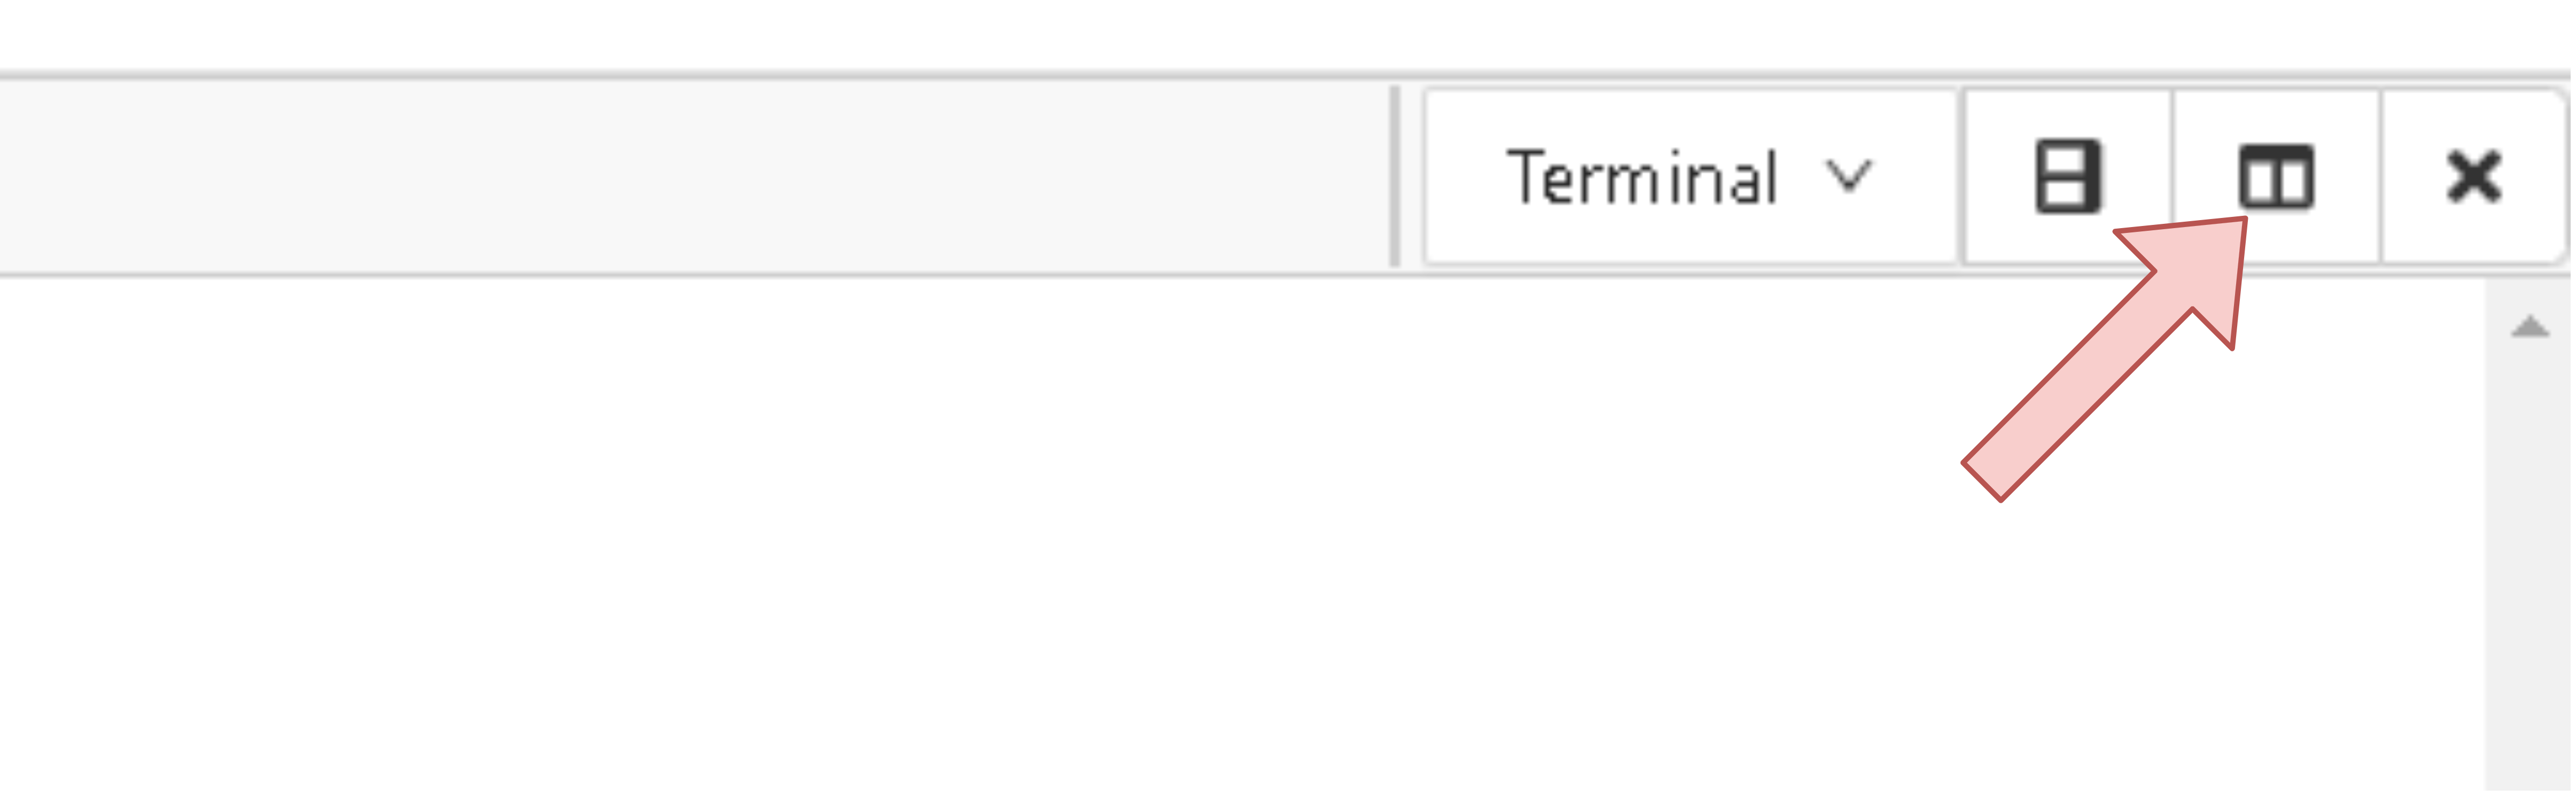
\includegraphics[width=7cm]{img/CoCalc2.png}
    \end{center}
    \item voilà, on peut commencer !
\end{enumerate}

\end{encadrecolore}
\newpage
\section*{Affichage statique des processus}
\begin{enumerate}
    \item Dans le terminal de gauche, taper \mintinline{bash}{ps -aux}.\\
    Que signifient les colonnes \texttt{PID}, \texttt{\%CPU}, \texttt{\%MEM} ?\\

    \item La colonne \texttt{STAT} indique l'état du processus, il suffit de regarder la première lettre : \texttt{R} pour \textit{Running}, \texttt{S} pour \texttt{Sleeping}, \tw{T} pour \tw{sTopped} par exemple.
        Dans le terminal de droite, tu vas créer un script \textsc{Python} nommé \texttt{inp.py} à l'aide de la commande \mintinline{bash}{nano} :
        \begin{enumerate}[--]
        	\item tape \mintinline{bash}{nano inp.py};
            \item dans l'éditeur, tape la seule ligne \mintinline{python}{a = input('En attente de texte : ')};
            \item enregistre en pressant \touche{CTRL} + \touche{o} puis \touche{Enter};
            \item quitte \texttt{nano} en pressant \touche{CTRL} + \touche{x};\\
        \end{enumerate}
        Exécute ce script en tapant \mintinline{bash}{python inp.py} puis laisse-le tourner.\\
        Dans le terminal de gauche, affiche la liste des processus.\\
        Dans quel état se trouve le processus \textsc{Python} ? Pourquoi ?\\

    \item Dans le terminal de droite, crée un script \textsc{Python} appelé \texttt{bcl.py} dans lequel il y aura une boucle infinie (sans mettre d'\mintinline{python}{input}, mais avec un \mintinline{python}{print}).\\
        Ensuite exécute-le, puis dans le terminal de gauche, affiche la liste des processus.\\
        Que remarques-tu ?\\

    \item Pour suspendre l'activité du processus (et arrêter le massacre), dans le terminal de droite presse \touche{CTRL} + \touche{z}.\\

    \item Selon \texttt{ps}, dans quel état se trouve le processus ?\\

    \item Pour réactiver le processus, tape \mintinline{bash}{fg} dans le terminal de droite.\\
            Pour l'arrêter définitivement, tape \touche{CTRL} + \touche{c}.\\

    \item Relance \texttt{bcl.py} à droite , puis, dans le terminal de gauche, affiche la liste des processus.\\
          Pour arrêter définitivement un processus, l'instruction est \mintinline{bash}{kill} suivi du \texttt{PID} du processus.\\
          Arrête \texttt{bcl.py}.
\end{enumerate}
\newpage
\section*{Affichage dynamique des processus et ressources}
\begin{enumerate}
	\item Dans le terminal de gauche, tape \mintinline{bash}{top}.\\
     Ce que tu obtiens est l'équivalent du gestionnaire des tâches de \textsc{Windows}.\\

     \item Dans le terminal de droite, écris un petit script appelé \mintinline{python}{bcl2.py} qui calcule
     $$1^4+2^4+\ldots+20\,000\,000^4$$
     Exécute-le et regarde l'état du processus dans le terminal de gauche. Comment interpréter la consommation CPU ?\\

     \item Modifie ce script
     \begin{enumerate}[--]
     	\item en ajoutant en première ligne \mintinline{python}{from time import sleep};
         \item en allant jusqu'à $10\,000$ au lieu de $20\,000\,000$;
         \item en rajoutant dans la boucle \mintinline{python}{sleep(0.001)} (dormir 1 milliseconde).
     \end{enumerate}
     Exécute ton script et regarde top. Quelles conclusions peux-tu en tirer ?
\end{enumerate}
\section*{Arbre des processus}
Tu peux fermer un des deux terminaux.\\

Comme expliqué dans le cours, un premier processus est d'abord créé par l'OS, puis c'est à partir de celui-ci que d'autres sont créés et ainsi de suite.\\
Le premier processus est celui qui a le plus petit PID.\\
\begin{enumerate}
	\item 	Quelle commande a lancé le premier processus ?
	\item 	Lorsque \texttt{top} est exécuté, on peut, en appuyant sur \touche{f} , ajouter des colonnes et en modifier l'ordre.\\
            Ajoute la colonne PPID de telle sorte qu'elle soit placée juste après PID.
     \item 	En regardant ces deux colonnes, reconstruis l'arborescence des processus.
     \item 	Tu peux quitter \texttt{top} et vérifier ton arborescence avec \texttt{pstree} (il manquera \texttt{top} mais il y aura un autre processus)...
     \end{enumerate}

\newpage
\section*{Observation de l'ordonnancement}
\begin{enumerate}
    \item Il est possible d'exécuter un processus en tâche de fond pour que le terminal « garde la main» en ajoutant une esperluette à la fin de la commande.\\
          Tapes \mintinline{bash}{python bcl2.py &}.\\
          Tu peux exécuter \mintinline{bash}{ps -aux} et constater que le processus est bien là et qu'il finit par se terminer.
	\item Enregistre le script suivant sous le nom \texttt{proc.py}
    \begin{pyc}
from os import getpid

pid = str(getpid()) # on récupère le n° de processus
print(f'---------------------------DEBUT PROCESSUS {pid}')
for i in range(1000):
    print(f'processus {pid} valeur {i}')
print(f'___________________________FIN PROCESSUS {pid}')
    \end{pyc}
    Exécute-le pour constater qu'il fonctionne.
    \item Exécute la commande \mintinline{bash}{python proc.py & python proc.py & python proc.py &} pour en lancer 3 instances.\\
        Recommence plusieurs fois (tu peux effacer l'écran avec \mintinline{bash}{clear}).\\

        Les 3 processus sont-ils exécutés à la suite les uns des autres ou bien y a-t-il chevauchement ?

        L'exécution simultanée des 3 processus se passe-t-elle de manière prévisible (on dit aussi déterministe) ?
\end{enumerate}

\end{document}